% Options for packages loaded elsewhere
\PassOptionsToPackage{unicode}{hyperref}
\PassOptionsToPackage{hyphens}{url}
\PassOptionsToPackage{dvipsnames,svgnames,x11names}{xcolor}
%
\documentclass[
  ignorenonframetext,
]{beamer}
\usepackage{pgfpages}
\setbeamertemplate{caption}[numbered]
\setbeamertemplate{caption label separator}{: }
\setbeamercolor{caption name}{fg=normal text.fg}
\beamertemplatenavigationsymbolsempty
% Prevent slide breaks in the middle of a paragraph
\widowpenalties 1 10000
\raggedbottom

\usepackage{amsmath,amssymb}
\usepackage{iftex}
\ifPDFTeX
  \usepackage[T1]{fontenc}
  \usepackage[utf8]{inputenc}
  \usepackage{textcomp} % provide euro and other symbols
\else % if luatex or xetex
  \usepackage{unicode-math}
  \defaultfontfeatures{Scale=MatchLowercase}
  \defaultfontfeatures[\rmfamily]{Ligatures=TeX,Scale=1}
\fi
\usepackage{lmodern}
\usetheme[]{AnnArbor}
\usecolortheme{dolphin}
\usefonttheme{structurebold}
\ifPDFTeX\else  
    % xetex/luatex font selection
\fi
% Use upquote if available, for straight quotes in verbatim environments
\IfFileExists{upquote.sty}{\usepackage{upquote}}{}
\IfFileExists{microtype.sty}{% use microtype if available
  \usepackage[]{microtype}
  \UseMicrotypeSet[protrusion]{basicmath} % disable protrusion for tt fonts
}{}
\makeatletter
\@ifundefined{KOMAClassName}{% if non-KOMA class
  \IfFileExists{parskip.sty}{%
    \usepackage{parskip}
  }{% else
    \setlength{\parindent}{0pt}
    \setlength{\parskip}{6pt plus 2pt minus 1pt}}
}{% if KOMA class
  \KOMAoptions{parskip=half}}
\makeatother
\usepackage{xcolor}
\newif\ifbibliography
\setlength{\emergencystretch}{3em} % prevent overfull lines
\setcounter{secnumdepth}{-\maxdimen} % remove section numbering


\providecommand{\tightlist}{%
  \setlength{\itemsep}{0pt}\setlength{\parskip}{0pt}}\usepackage{longtable,booktabs,array}
\usepackage{calc} % for calculating minipage widths
\usepackage{caption}
% Make caption package work with longtable
\makeatletter
\def\fnum@table{\tablename~\thetable}
\makeatother
\usepackage{graphicx}
\makeatletter
\def\maxwidth{\ifdim\Gin@nat@width>\linewidth\linewidth\else\Gin@nat@width\fi}
\def\maxheight{\ifdim\Gin@nat@height>\textheight\textheight\else\Gin@nat@height\fi}
\makeatother
% Scale images if necessary, so that they will not overflow the page
% margins by default, and it is still possible to overwrite the defaults
% using explicit options in \includegraphics[width, height, ...]{}
\setkeys{Gin}{width=\maxwidth,height=\maxheight,keepaspectratio}
% Set default figure placement to htbp
\makeatletter
\def\fps@figure{htbp}
\makeatother
% definitions for citeproc citations
\NewDocumentCommand\citeproctext{}{}
\NewDocumentCommand\citeproc{mm}{%
  \begingroup\def\citeproctext{#2}\cite{#1}\endgroup}
\makeatletter
 % allow citations to break across lines
 \let\@cite@ofmt\@firstofone
 % avoid brackets around text for \cite:
 \def\@biblabel#1{}
 \def\@cite#1#2{{#1\if@tempswa , #2\fi}}
\makeatother
\newlength{\cslhangindent}
\setlength{\cslhangindent}{1.5em}
\newlength{\csllabelwidth}
\setlength{\csllabelwidth}{3em}
\newenvironment{CSLReferences}[2] % #1 hanging-indent, #2 entry-spacing
 {\begin{list}{}{%
  \setlength{\itemindent}{0pt}
  \setlength{\leftmargin}{0pt}
  \setlength{\parsep}{0pt}
  % turn on hanging indent if param 1 is 1
  \ifodd #1
   \setlength{\leftmargin}{\cslhangindent}
   \setlength{\itemindent}{-1\cslhangindent}
  \fi
  % set entry spacing
  \setlength{\itemsep}{#2\baselineskip}}}
 {\end{list}}
\usepackage{calc}
\newcommand{\CSLBlock}[1]{\hfill\break\parbox[t]{\linewidth}{\strut\ignorespaces#1\strut}}
\newcommand{\CSLLeftMargin}[1]{\parbox[t]{\csllabelwidth}{\strut#1\strut}}
\newcommand{\CSLRightInline}[1]{\parbox[t]{\linewidth - \csllabelwidth}{\strut#1\strut}}
\newcommand{\CSLIndent}[1]{\hspace{\cslhangindent}#1}


% logo
\titlegraphic{
\includegraphics[width=4cm]{000_logos/logo-blue-vertical}}
\logo{\ifnum\thepage>1
\includegraphics[width=0.5cm]{000_logos/logo-blue-vertical}\fi}

% UMNG: Manual de image institucional

% Colors

% Umng
\definecolor{yellow}{HTML}{fdc600}
\definecolor{red}{HTML}{ee2a24}

% Estudios a Distancia
\definecolor{blue1}{HTML}{12245b}
\definecolor{blue2}{HTML}{767ca6}
\definecolor{blue3}{HTML}{cad2ec}

% Modify items
\setbeamercolor{palette primary}{bg=blue3}
\setbeamercolor{palette tertiary}{bg=blue1}
\setbeamercolor{frametitle}{bg=yellow}

% Hyperlinks
\hypersetup{
  linkcolor=red,
  citecolor=red
}

\makeatletter
\@ifpackageloaded{caption}{}{\usepackage{caption}}
\AtBeginDocument{%
\ifdefined\contentsname
  \renewcommand*\contentsname{Table of contents}
\else
  \newcommand\contentsname{Table of contents}
\fi
\ifdefined\listfigurename
  \renewcommand*\listfigurename{List of Figures}
\else
  \newcommand\listfigurename{List of Figures}
\fi
\ifdefined\listtablename
  \renewcommand*\listtablename{List of Tables}
\else
  \newcommand\listtablename{List of Tables}
\fi
\ifdefined\figurename
  \renewcommand*\figurename{Figure}
\else
  \newcommand\figurename{Figure}
\fi
\ifdefined\tablename
  \renewcommand*\tablename{Table}
\else
  \newcommand\tablename{Table}
\fi
}
\@ifpackageloaded{float}{}{\usepackage{float}}
\floatstyle{ruled}
\@ifundefined{c@chapter}{\newfloat{codelisting}{h}{lop}}{\newfloat{codelisting}{h}{lop}[chapter]}
\floatname{codelisting}{Listing}
\newcommand*\listoflistings{\listof{codelisting}{List of Listings}}
\makeatother
\makeatletter
\makeatother
\makeatletter
\@ifpackageloaded{caption}{}{\usepackage{caption}}
\@ifpackageloaded{subcaption}{}{\usepackage{subcaption}}
\makeatother

\ifLuaTeX
\usepackage[bidi=basic]{babel}
\else
\usepackage[bidi=default]{babel}
\fi
\babelprovide[main,import]{english}
% get rid of language-specific shorthands (see #6817):
\let\LanguageShortHands\languageshorthands
\def\languageshorthands#1{}
\ifLuaTeX
  \usepackage{selnolig}  % disable illegal ligatures
\fi
\usepackage{bookmark}

\IfFileExists{xurl.sty}{\usepackage{xurl}}{} % add URL line breaks if available
\urlstyle{same} % disable monospaced font for URLs
\hypersetup{
  pdftitle={Ethics in Negotiation},
  pdfauthor={Luis Francisco Gómez López},
  pdflang={en},
  colorlinks=true,
  linkcolor={Maroon},
  filecolor={Maroon},
  citecolor={Blue},
  urlcolor={Blue},
  pdfcreator={LaTeX via pandoc}}


\title{Ethics in Negotiation}
\author{Luis Francisco Gómez López}
\date{2024-07-27}
\institute{FAEDIS}

\begin{document}
\frame{\titlepage}

\renewcommand*\contentsname{Table of contents}
\begin{frame}[allowframebreaks]
  \frametitle{Table of contents}
  \tableofcontents[hideallsubsections]
\end{frame}

\section{Please Read Me}\label{please-read-me}

\begin{frame}{}
\phantomsection\label{section}
\begin{itemize}
\item
  Check the message \textbf{Welcome greeting} published in the News
  Bulletin Board.
\item
  Dear student please edit your profile uploading a photo where your
  face is clearly visible.
\item
  The purpose of the virtual meetings is to answer questions and not to
  make a summary of the study material.
\item
  This presentation is based on
  (\citeproc{ref-lewicki_negociacion_2024}{Lewicki, Barry, and Saunders
  2024, chap. 5})
\end{itemize}
\end{frame}

\section{Purpose}\label{purpose}

\begin{frame}{}
\phantomsection\label{section-1}
Explore and understand the ethical standards commonly accepted in a
negotiation process in order to detect and deal with deceptive tactics.
\end{frame}

\section{Ethics and its relationship with
negotiation}\label{ethics-and-its-relationship-with-negotiation}

\begin{frame}{}
\phantomsection\label{section-2}
\begin{itemize}
\item
  Ethics is understand as the social standards that are apply to examine
  what is right or wrong in a specific situation or a process to
  establish such standards
  (\citeproc{ref-lewicki_negociacion_2024}{Lewicki, Barry, and Saunders
  2024, chap. 5}, p 136).
\item
  The ethical considerations in a negotiation are related to how the
  exchange of information occurs
  (\citeproc{ref-lewicki_ethical_1998}{Lewicki and Robinson 1998}).

  \begin{itemize}
  \tightlist
  \item
    Because the exchange of information in the negotiation process is
    vital, the analysis of ethics is associated with examining whether
    or not there is a dishonest communication.
  \end{itemize}
\end{itemize}
\end{frame}

\begin{frame}{}
\phantomsection\label{section-3}
\begin{itemize}
\tightlist
\item
  To evaluate how ethical the strategies and tactics are in a
  negotiation, 4 standards can be used
  (\citeproc{ref-lewicki_negociacion_2024}{Lewicki, Barry, and Saunders
  2024, chap. 5}, p 118):
\end{itemize}

\begin{figure}

\centering{

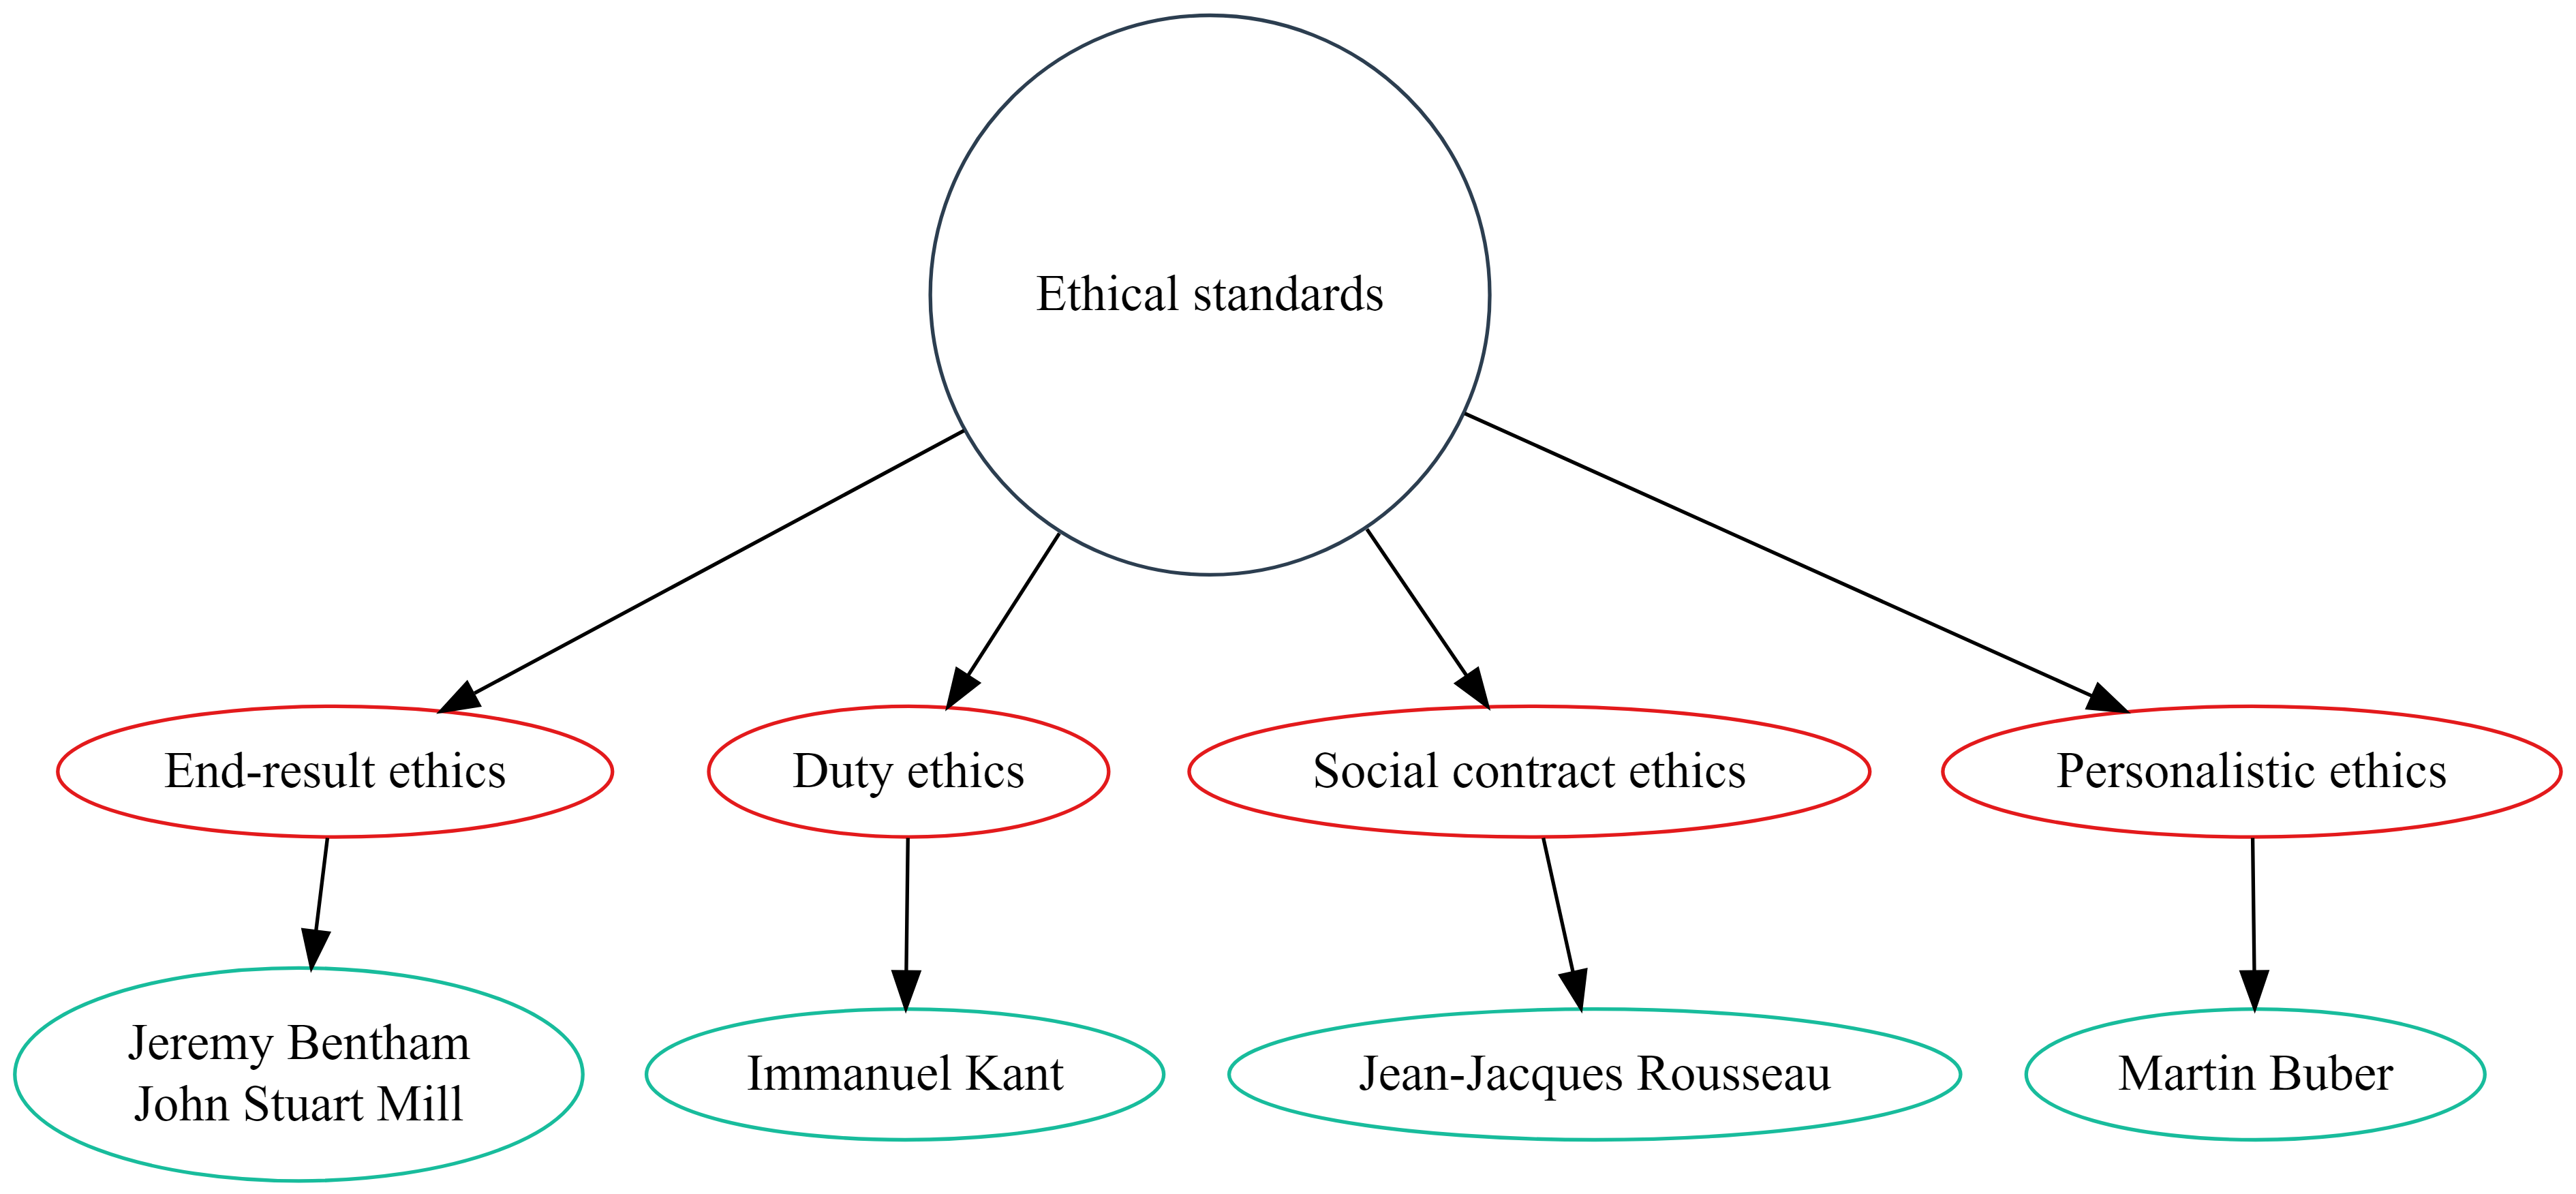
\includegraphics[width=4.5in,height=2.5in]{008_ethics_files/figure-beamer/dot-figure-1.png}

}

\caption{\label{fig-approaches-to-ethical-reasoning}Approaches to
ethical reasoning to evaluate strategies and tactics in a negotiation
(\citeproc{ref-lewicki_negociacion_2024}{Lewicki, Barry, and Saunders
2024}, pp 140)}

\end{figure}%
\end{frame}

\section{Ethically ambiguous tactics}\label{ethically-ambiguous-tactics}

\begin{frame}{}
\phantomsection\label{section-4}
\begin{itemize}
\item
  There are tactics that are not ethical and that can be quickly
  identified, such as stealing confidential data from the counterpart.

  \begin{itemize}
  \tightlist
  \item
    These types of tactics must be removed from the negotiator's
    toolbox.
  \end{itemize}
\item
  However, in the context of negotiation there are gray areas. These
  gray areas are known as ethically ambiguous tactics within the theory
  of negotiation.

  \begin{itemize}
  \tightlist
  \item
    These tactics are related to what the negotiators say or what they
    claim they will do concerning what they really do.
  \end{itemize}
\end{itemize}
\end{frame}

\begin{frame}{}
\phantomsection\label{section-5}
\begin{itemize}
\item
  Gray areas within a negotiating context regarding ethically ambiguous
  tactics are presented due to the 2 dilemmas a negotiator faces:

  \begin{itemize}
  \item
    Dilemma of honesty

    \begin{itemize}
    \tightlist
    \item
      How much truth should be revealed to the counterpart?
    \end{itemize}
  \item
    Dilemma of trust

    \begin{itemize}
    \tightlist
    \item
      How much should a negotiator believe what the counterpart says?
    \end{itemize}
  \end{itemize}
\end{itemize}
\end{frame}

\begin{frame}{}
\phantomsection\label{section-6}
\begin{figure}

\centering{

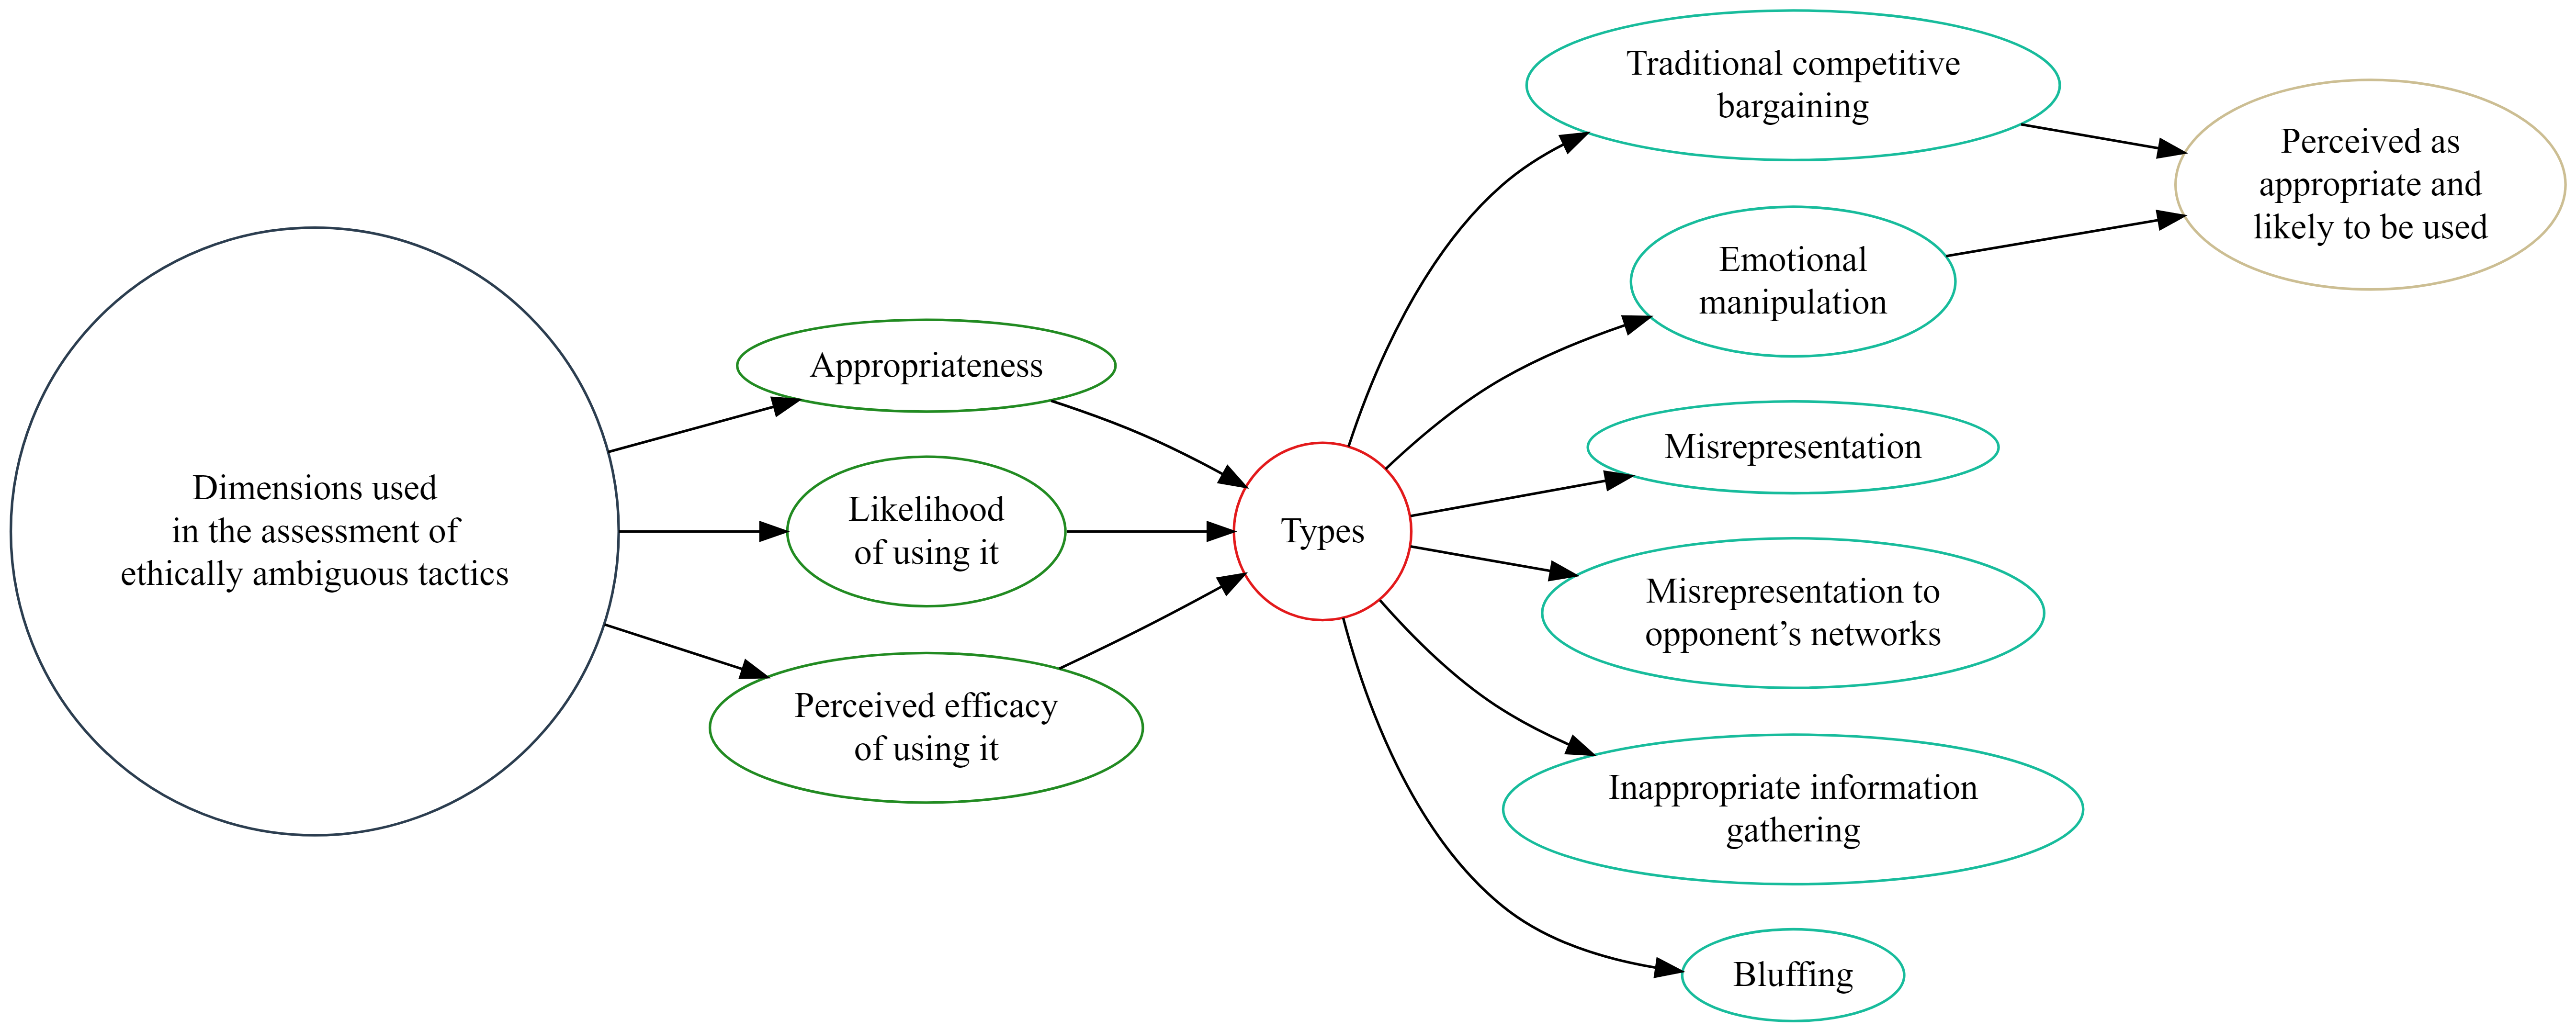
\includegraphics[width=4.5in,height=2.5in]{008_ethics_files/figure-beamer/dot-figure-5.png}

}

\caption{\label{fig-types-ethically-ambiguous-tactics}Types of ethically
ambiguous tactics (\citeproc{ref-lewicki_negociacion_2024}{Lewicki,
Barry, and Saunders 2024}, p 148)}

\end{figure}%
\end{frame}

\section{Motives and consequences of using deceptive
tactics}\label{motives-and-consequences-of-using-deceptive-tactics}

\begin{frame}{}
\phantomsection\label{section-7}
\begin{figure}

\centering{

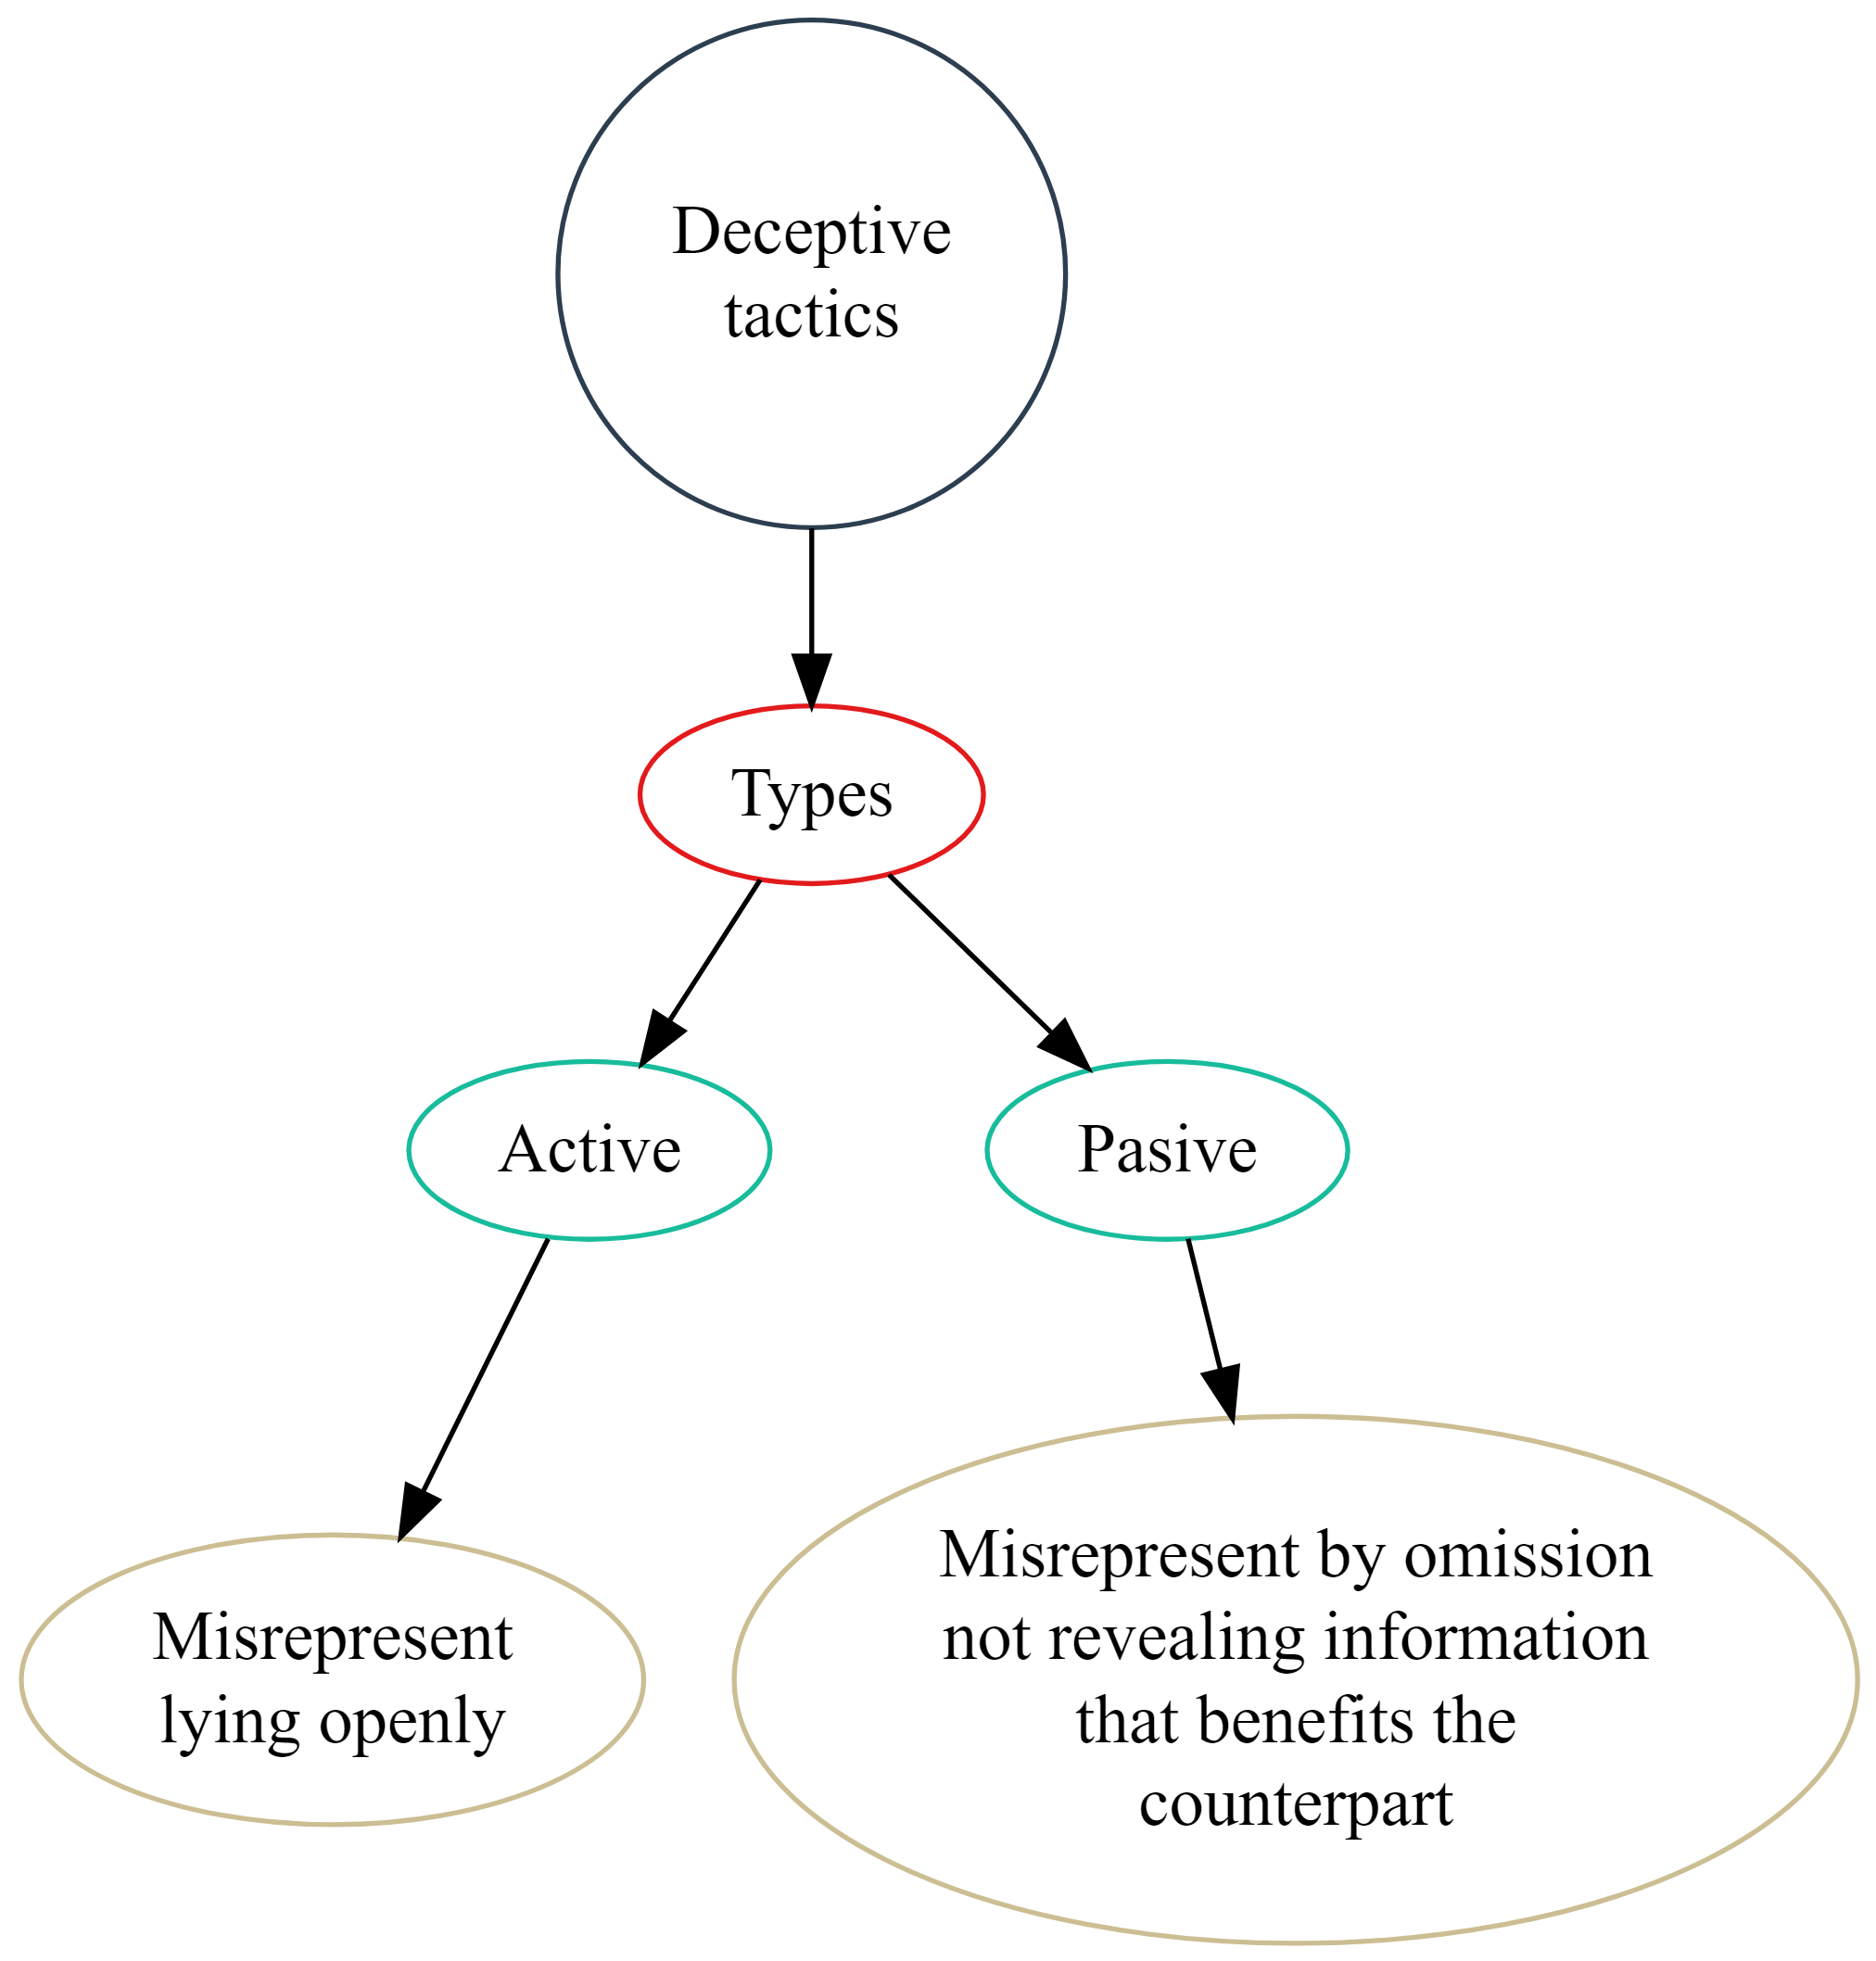
\includegraphics[width=4.5in,height=2.5in]{008_ethics_files/figure-beamer/dot-figure-4.png}

}

\caption{\label{fig-use-of-deceptive-tactics}Use of deceptive tactics
(\citeproc{ref-lewicki_negociacion_2024}{Lewicki, Barry, and Saunders
2024}, p 151)}

\end{figure}%
\end{frame}

\begin{frame}{}
\phantomsection\label{section-8}
\begin{itemize}
\item
  Why do negotiators use deceptive tactics in the context of a
  negotiation?

  \begin{itemize}
  \item
    Need to acquire greater power through the manipulation of
    information to get closer to the target point
  \item
    Use of a more competitive negotiation style\footnote<.->{This aspect
      generates a greater probability of using this type of tactics}
  \end{itemize}
\end{itemize}
\end{frame}

\begin{frame}{}
\phantomsection\label{section-9}
\begin{figure}

\centering{

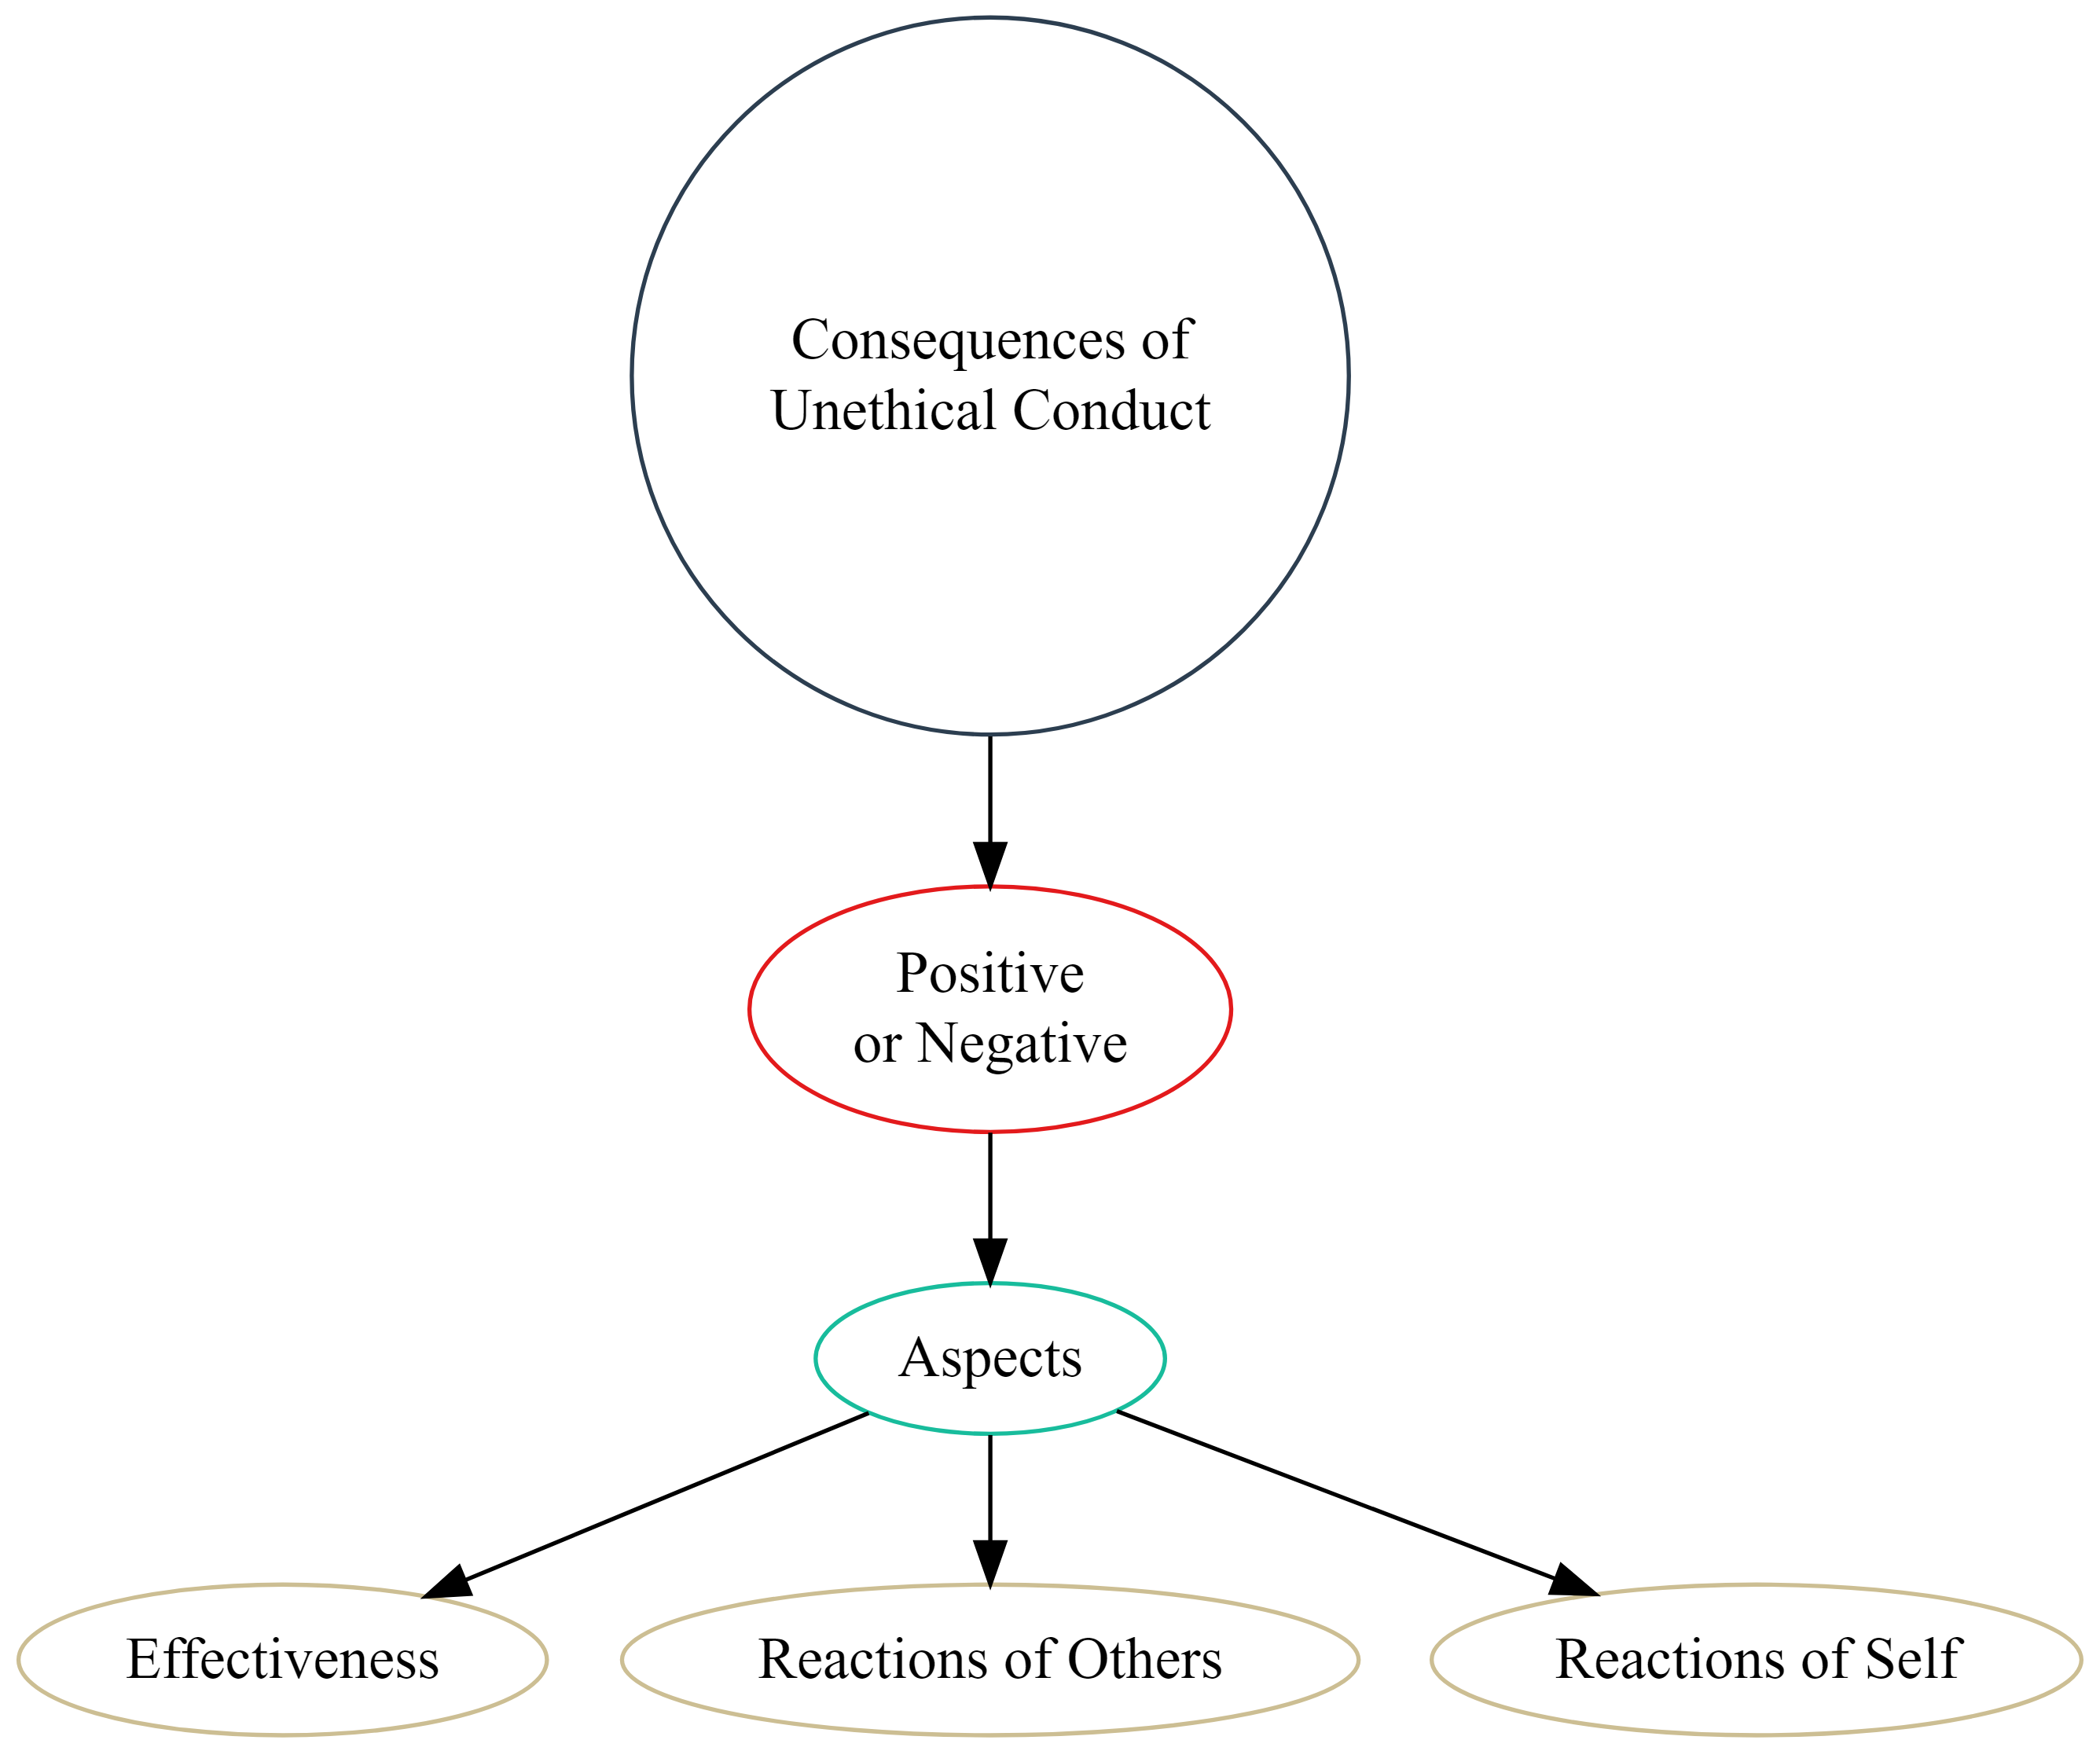
\includegraphics[width=4.5in,height=2.5in]{008_ethics_files/figure-beamer/dot-figure-3.png}

}

\caption{\label{fig-consequences-of-unethical-conduct}Consequences of
unethical conduct (\citeproc{ref-lewicki_negociacion_2024}{Lewicki,
Barry, and Saunders 2024}, pp 155-158)}

\end{figure}%
\end{frame}

\begin{frame}{}
\phantomsection\label{section-10}
\begin{itemize}
\item
  \textbf{Effectiveness}

  \begin{itemize}
  \item
    Deceptive tactics generate \textbf{positive consequences} when the
    outcome of the negotiation improves compared to whether a negotiator
    had acted ethically and if the conduct is not punished where the
    consequences materialize in the short run.
  \item
    Deceptive tactics generate \textbf{negative consequences} because
    the reputation of the negotiator is damaged where the consequences
    materialize in the future.
  \end{itemize}
\end{itemize}
\end{frame}

\begin{frame}{}
\phantomsection\label{section-11}
\begin{itemize}
\item
  \textbf{Reactions of Others}

  \begin{itemize}
  \item
    Deceptive tactics generate \textbf{positive consequences} only if
    constituents, indirect actors or interest observers considered
    appropriate to use this type of tactics\footnote<.->{This is my own
      personal opinion and it is not mentioned in
      (\citeproc{ref-lewicki_negociacion_2024}{Lewicki, Barry, and
      Saunders 2024, chap. 5})}.
  \item
    Deceptive tactics generate \textbf{negative consequences} because
    retaliations occur directly from the counterpart and possibly from
    the constituents, indirect actors or interest observers if they
    consider that the tactic used is inappropriate\footnote<.->{As a
      personal opinion in the case of the indirect actors or interest
      observers the retaliation is materialize through a social
      sanction.}.
  \end{itemize}
\end{itemize}
\end{frame}

\begin{frame}{}
\phantomsection\label{section-12}
\begin{itemize}
\item
  \textbf{Reactions of Self}

  \begin{itemize}
  \item
    Deceptive tactics generate \textbf{positive consequences} only if
    the negotiator does not suffer from guilt, remorse or discomfort.
  \item
    Deceptive tactics generate \textbf{negative consequences} when the
    negotiator suffers from guilt, remorse or discomfort for having used
    these tactics\footnote<.->{This issue directly affects the
      negotiation since the negotiator is willing to make greater
      concessions to the counterpart to compensate for using deceptive
      tactics.}
  \end{itemize}
\end{itemize}
\end{frame}

\section{Dealing with the use of deceptive tactics by the
counterpart}\label{dealing-with-the-use-of-deceptive-tactics-by-the-counterpart}

\begin{frame}{}
\phantomsection\label{section-13}
\begin{figure}

\centering{

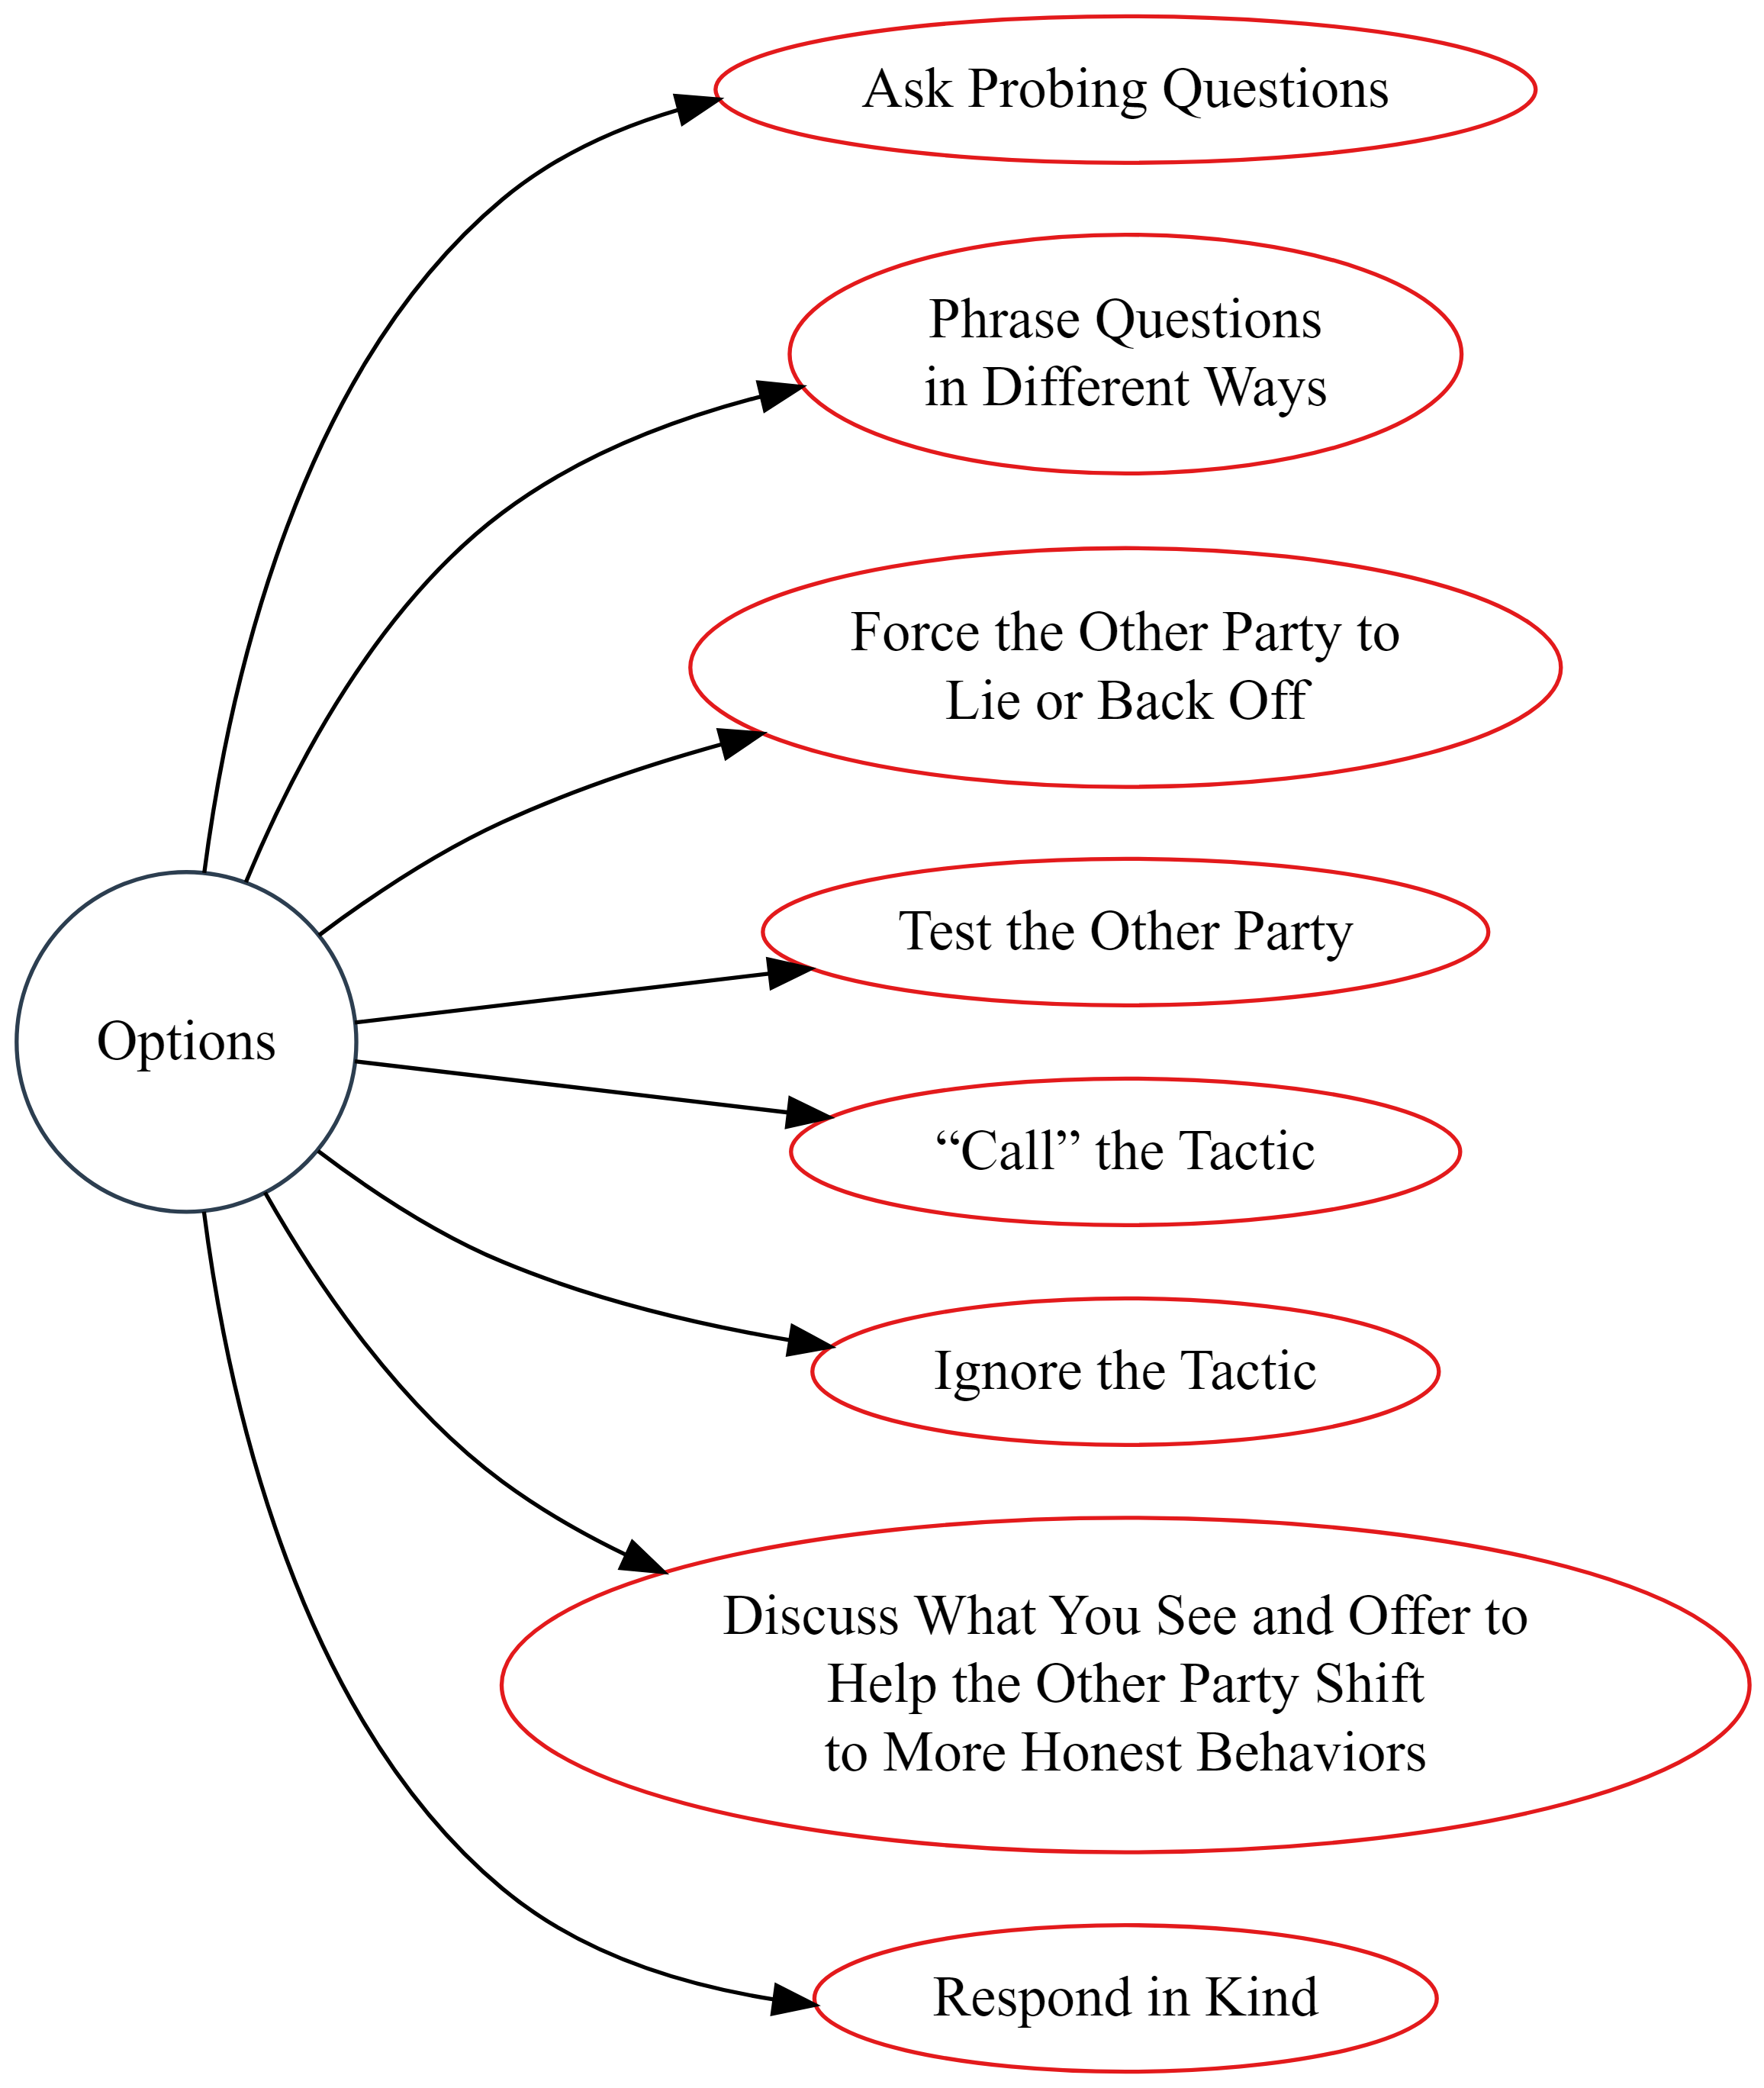
\includegraphics[width=4.5in,height=2.5in]{008_ethics_files/figure-beamer/dot-figure-2.png}

}

\caption{\label{fig-dealing-with-deceptive-tactics}Dealing with
deceptive tactics by the counterpart
(\citeproc{ref-lewicki_negociacion_2024}{Lewicki, Barry, and Saunders
2024}, pp 172-174)}

\end{figure}%
\end{frame}

\begin{frame}{}
\phantomsection\label{section-14}
\begin{itemize}
\item
  \textbf{My personal opinion}:

  \begin{itemize}
  \item
    Read the article (\citeproc{ref-adler_negotiating_2007}{Adler
    2007}):

    \begin{itemize}
    \item
      Before the Bargaining Begins
    \item
      During the Bargaining Process
    \end{itemize}
  \item
    I think the best approach is to follow the recommendations in the
    section \textbf{Before the Bargaining Begins} because they are
    carried out during the planning stage of a negotiation where there
    is more time and information that can be collected in order to
    respond adequately to deceptive tactics.
  \end{itemize}
\end{itemize}
\end{frame}

\section{Acknowledgments}\label{acknowledgments}

\begin{frame}{}
\phantomsection\label{section-15}
\begin{itemize}
\item
  To my family that supports me
\item
  To the taxpayers of Colombia and the
  \href{https://www.umng.edu.co/estudiante}{\textbf{UMNG students}} who
  pay my salary
\item
  To the \href{https://www.business-science.io/}{\textbf{Business
  Science}} and \href{https://www.rfordatasci.com/}{\textbf{R4DS Online
  Learning}} communities where I learn
  \href{https://www.r-project.org/about.html}{\textbf{R}} and
  \href{https://www.python.org/about/}{\textbf{\(\pi\)-thon}}
\item
  To the \href{https://www.r-project.org/contributors.html}{\textbf{R
  Core Team}}, the creators of
  \href{https://rstudio.com/products/rstudio/}{\textbf{RStudio IDE}},
  \href{https://quarto.org/}{\textbf{Quarto}} and the authors and
  maintainers of the packages
  \href{https://CRAN.R-project.org/package=tinytex}{\textbf{tinytex}}
  for allowing me to access these tools without paying for a license
\item
  To the \href{https://www.kernel.org/category/about.html}{\textbf{Linux
  kernel community}} for allowing me the possibility to use some
  \href{https://static.lwn.net/Distributions/}{\textbf{Linux
  distributions}} as my main
  \href{https://en.wikipedia.org/wiki/Operating_system}{\textbf{OS}}
  without paying for a license
\end{itemize}
\end{frame}

\section*{References}\label{references}
\addcontentsline{toc}{section}{References}

\begin{frame}[allowframebreaks]{References}
\phantomsection\label{refs}
\begin{CSLReferences}{1}{0}
\bibitem[\citeproctext]{ref-adler_negotiating_2007}
Adler, Robert S. 2007. {``Negotiating with Liars.''} \emph{MIT Sloan
Management Review} 48 (4): 69--79.

\bibitem[\citeproctext]{ref-lewicki_negociacion_2024}
Lewicki, Roy J., Bruce Barry, and David M. Saunders. 2024.
\emph{Negociación}. 9th ed. McGraw-Hill Education.
\url{https://www-ebooks7-24-com.ezproxy.umng.edu.co/?il=40562}.

\bibitem[\citeproctext]{ref-lewicki_ethical_1998}
Lewicki, Roy J., and Robert J. Robinson. 1998. {``Ethical and
{Unethical} {Bargaining} {Tactics}: {An} {Empirical} {Study}.''}
\emph{Journal of Business Ethics} 18 (2): 211--28.
\url{https://doi.org/10.1023/A:1005719122519}.

\end{CSLReferences}
\end{frame}




\end{document}
